\documentclass[12pt]{article}

\usepackage{sbc-template}


\usepackage{graphicx}
\usepackage{pythontex} 
\usepackage[brazil]{babel}   
\usepackage[utf8]{inputenc}  
\usepackage{circuitikz}
\usepackage{siunitx}
\usepackage{gensymb}


\sloppy

\title{Análise do Circuito RC}

\author{Pedro Henrique Gomes\inst{1}, Sarah Pereira Cerqueira\inst{2} }


\address{Departamento de Tecnologia (DTEC) -- Universidade Estadual de Feira de Santana
  (UEFS)\\
  Caixa Postal 252 e 294 -- 44036-900 -- Feira de Santana -- BA -- Brazil
  \email{ peuh\_fsa@hotmail.com,
  sarahecomp@gmail.com}
}

\begin{document} 

\maketitle

\begin{resumo}
O presente documento faz uma análise do circuito RC em série  no domínio da frequência
\end{resumo}

 \section{Introdução}
 O circuito resistor-capacito (RC), é um dos filtros eletrônicos mais simples e básico da eletrônica. Ele consiste em um capacitor e um resistor ligados em série ou paralelo, alimentados por uma fonte de tensão. 
 
 Diferente de circuitos puramente resistivos, cuja aplicação das leis de Kirchhoff resulta numa equação algébrica, a aplicação das leis de Kirchhorff em um circuito RC produz uma equação diferencial de primeira ordem, que é mais difícil de resolver do que uma algébrica. 
 
 Ao alimentar o circuito RC com uma fonte senoidal de amplitude constante, variando a frequência obtemos a resposta em frequência do circuito, que pode ser considerada uma descrição completa do compotamento em regime estacionário senoidal de um circuito em função da frequência. 
 
 Neste trabalho será feita uma análise do ciruito RC em série, no domínio da frequência apresentando sua  função transferência.
 
 \section{ Metodologia}


\subsection{Diagrama do Circuito}

%DESENHO DO CIRCUITO
\begin{center}
\begin{circuitikz}[scale=1.6, transform shape][american voltages]
\draw 
(0,0){to[american voltage source, invert, l=$Vi$, color=red] (0,2) }
 to[R, l=$R$, i=$i$] (2,2)
 to[capacitor, v^>=$Vo$] (2,0) -- (0,0)
 ;\end{circuitikz}
 \end{center}

 %ANÁLISE DO CIRCUITO

 
 \subsection{Análise do Circuito}

Sendo o sinal de entrada uma tensão elétrica doméstica comum ( amplitude de 110V, frequência de 120Hz) :
\begin{equation}
Vi(t) = 110.\sqrt{2}.sin(120t + 0\degree)  [V]\\
\end{equation}

Em forma fasorial:
\begin{equation}
Vi(jw) = 110\angle 0\degree
\end{equation}

A reatância e a Indutância num capacitor podem ser descritas por:

\begin{equation}
Xc = \frac{1}{w.C}  [\si{\ohm}]\\
\end{equation}

\begin{equation}
Zc = Xc.j [\si{\ohm}]\\
\end{equation}

logo:

\begin{equation}
Zc = \frac{j}{w.C} [\si{\ohm}]\\
\end{equation}

Aplicando o divisor de Tensão:

\begin{equation}
Vo(w)=\frac{Zc.Vi}{Zc+Zr}[V]
\end{equation}

Sabemos que a impedância Zr no resistor vale:

\begin{equation}
Zr= R [\si{\ohm}]
\end{equation}


Agora substituindo (5) em (6), 

\begin{equation}
Vo(w)=\frac{\frac{j.Vi}{w.C}}{\frac{j}{w.C} + R} [V]
\end{equation}

Simplificando esse resultado, temos: 

\begin{equation}
Vo(w)=\frac{1.Vi}{1+jwRC}[V]
\end{equation}

Portanto, a resposta em frequência desse circuito é expressa por:
\begin{equation}
\frac{Vo(w)}{Vi(w)}=\frac{1}{1+jwRC}
\end{equation}

Como solicitado, consideraremos a constante de tempo R.C = 1, então temos:

\begin{equation}
\frac{Vo(w)}{Vi(w)}=\frac{1}{1+j.w}
\end{equation}

Obs: Esta função também pode ser escrita, substituindo s=j.w, da seguinte maneira:
 
\begin{equation}
\frac{Vo(s)}{Vi(s)}=\frac{1}{1+\textit{s}}
\end{equation}


Como todo número complexo, resposta em frequência também possui notação fasorial, a partir de seu módulo e fase:

\begin{equation}
\left|\frac{Vo(jw)}{Vi(jw)} \right|= \frac{1\angle 0\degree}{\sqrt{1^2+(wRC)^2}\angle arctg(\frac{wRC}{1})} 
\end{equation}


%ANÁLISE ASSINTÓTICA DO CIRCUITO
 \section{Análise Assintótica do Circuito}     
Uma vez conhecido o módulo da resposta em frequência, é possível realizar uma análise assintótica da mesma, a qual será dividia em 4 etapas. A partir delas, é possível identificar o comportamento da função aferida anteriormente, além do ganho de tensão em determinado ponto, o qual é expresso por:

\begin{equation}
G = 20log(\left|\frac{Vo}{Vi} \right|) [dB]
\end{equation}


\subsection{Ponto de Origem (w = 0 rad/s)}

O ponto de origem, equivale ao nível DC do sinal, onde sua frequência é zero.

\begin{equation}
\left|\frac{Vo(jw)}{Vi(jw)} \right| = \frac{1}{\sqrt{1^2+(wRC)^2}} = 1
\end{equation}

\begin{equation}
\left|Vo(jw)|\right = \left|Vi(jw)| \right 
\end{equation}

Portanto, pode-se notar que a tensão de Entrada será igual a tensão de saída, em módulo.

Quanto ao ganho de tensão:

\begin{equation}
G = 20.log(1) = 0dB
\end{equation}

Visto isso, pode-se perceber que nesse caso não há ganho nem perda de tensão.

\subsection{Ponto de Corte (w = 1/RC rad/s)}

Na ponto de corte, ocorre uma queda na frequência de saída para 0,707 da frequência de entrada.  

\begin{equation}
\left|\frac{Vo(jw)}{Vi(jw)} \right| = \frac{1}{\sqrt{1^2+(wRC)^2}} = \frac{1}{\sqrt{2}} = 0,707
\end{equation}

Quanto ao ganho de tensão:

\begin{equation}
G = 20.log(0,707) = -3,01dB
\end{equation}


\subsection{Uma oitava acima do ponto de corte (w = 2/RC rad/s)}
Uma oitava acima do ponto de corte, significa que a frequência de corte será dobrada. Nesse momento, ocorre uma queda na frequência de saída para 0,577 da frequência de entrada.  


\begin{equation}
\left|\frac{Vo(jw)}{Vi(jw)} \right| = \frac{1}{\sqrt{1^2+(wRC)^2}} = \frac{1}{\sqrt{3}} = 0,577
\end{equation}

Quanto ao ganho de tensão:

\begin{equation}
G = 20.log(0,577) = - 4,78dB
\end{equation}

\subsection{Uma década acima do ponto de corte (w = 10/RC rad/s)}

Uma oitava acima do ponto de corte, significa que a frequência de corte será 10 vezes maior do que a frequência de corte. Nesse momento, ocorre uma queda na frequência de saída para 0,301 da frequência de entrada.  


\begin{equation}
\left|\frac{Vo(jw)}{Vi(jw)} \right| = \frac{1}{\sqrt{1^2+(wRC)^2}} = \frac{1}{\sqrt{11}} = 0,301
\end{equation}

Quanto ao ganho de tensão:

\begin{equation}
G = 20.log(0,301) = -10,43dB
\end{equation}


\section{Conclusão}
A função transferência de um circuito é a razão, dependende da frequência, de uma saída para uma entrada, e é útil para encontrar a resposta em frequência de um circuito. No caso do circuito RC análisado, a equação (12) indica a função transferência correspondente ao ganho de tensão.

O gráfico da Figura 1 exibe o comportamento da equação (12), onde o eixo das abicissas é variável independente  \textit{s}. 

\begin{figure}[h]
\centering
\begin{pycode}

from pyx import *

g = graph.graphxy(width=8)
g.plot(graph.data.function("y(x)=1/(x+1)", min=0, max=50))
g.writePDFfile("function")
print (r'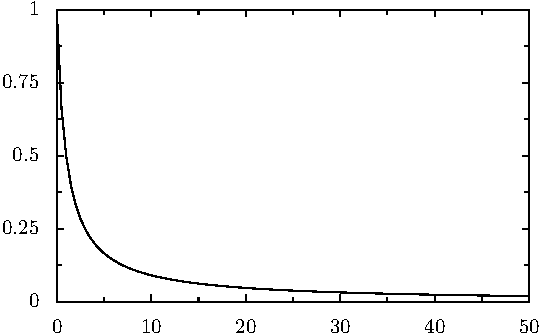
\includegraphics{function}')
\end{pycode}
\caption{$\frac{Vo(s)}{Vi(s)}=$$\frac{1}{1+s}$}
\end{figure}

Como a saída do circuito é obtida pelo capacitor, o circuito se configura como um filtro passa-baixas padrão. Para frequência igual a zero, o ganho em tensão é 1, e para frequencia no infinito o ganho em tensão é 0.

Outra conclusão a qual é possível chegar, desta vez a partir da análise assintótica, é que o comportamento da resposta em frequência na medida em que tal frequência varia de 0 a infinito, tende a se comportar de maneira descrescente, assim como previsto na análise matemática, e no gráfico acima.

Em relação ao ganho em decibéis, percebe-se uma perda de tensão em escala logarítmica, na medida em que a razão entre as frequências de entrada e saída diminui.

\bibliographystyle{sbc}
\bibliography{sbc-template}

\end{document}
